\documentclass[12pt]{article}

% 基本包
\usepackage{xeCJK}
\usepackage{graphicx}
\usepackage{amsmath}
\usepackage{amssymb}
\usepackage{hyperref}
\usepackage{geometry}
\usepackage{setspace}
\usepackage{enumitem}
\usepackage{booktabs}
\usepackage{multirow}
\usepackage{float}
\usepackage{subcaption}
\usepackage{listings}
\usepackage{xcolor}
\usepackage{algorithm}
\usepackage{algorithmic}
\usepackage[backend=bibtex,style=numeric]{biblatex}
\addbibresource{references.bib}

% 設置中文字體
\setCJKmainfont{Heiti TC}
\setCJKsansfont{Heiti TC}
\setCJKmonofont{Heiti TC}

% 統一設定列表間距
\setlist{noitemsep,topsep=4pt}

% 頁面設置
\geometry{a4paper, margin=1in}
\onehalfspacing
\setlength{\parindent}{2em}  % 設定段落第一行縮排為兩個中文字寬度

% 超連結設置
\hypersetup{
    colorlinks=true,
    linkcolor=black,
    filecolor=magenta,      
    urlcolor=cyan,
    pdftitle={pdf title},
    pdfauthor={Raiso Liu},
    pdfsubject={pdf subject},
    pdfkeywords={pdf keywords}
}

% 代碼塊設置
\lstset{
    frame=none,
    breaklines=true,
    postbreak=\raisebox{0ex}[0ex][0ex]{\ensuremath{\hookrightarrow\space}},
    basicstyle=\ttfamily\scriptsize,
    keywordstyle=\color{blue},
    stringstyle=\color{red},
    commentstyle=\color{green!60!black},
    showstringspaces=false,
    backgroundcolor=\color{gray!5},
    xleftmargin=0em,
    xrightmargin=0em,
    linewidth=0.95\textwidth,
    captionpos=b
}

% 設定所有 listings 環境
\renewcommand{\lstlistingname}{Code}
\renewcommand{\lstlistlistingname}{Code List}

% 文檔信息
\title{MaskGIT Report}
\author{劉宇舜\\Department of Computer Science and Information Engineering\\National Yang Ming Chiao Tung University}
\date{\today}

\begin{document}

% 添加封面
\begin{titlepage}
    \begin{center}
        \vspace*{2cm}
        
        \Huge
        \textbf{Generative Models}
        
        \vspace{1.5cm}
        
        \Large
        \textbf{劉宇舜 Yu-Shun Liu}
        
        \vspace{1cm}
        
        \large
        Student ID: 413551030
        
        \vspace{2cm}
        
        \large
        Department of Computer Science and Information Engineering\\
        National Yang Ming Chiao Tung University
        
        \vspace{1cm}
        
        \large
        Course: Deep Learning
        
        \vspace{1cm}
        
        \large
        \today
        
    \end{center}
\end{titlepage} 

% 添加目錄
\setcounter{tocdepth}{2}
\tableofcontents
\newpage

% 添加報告內容
\section{Introduction}


這次的目標是學會使用 conditional 的資訊來生成圖片,透過降噪的過程,學會如何從一個模糊的圖片,一步一步的恢復成一個清晰的圖片,並且學會如何使用 conditional 的資訊,來生成我想要的圖片。

這篇作業我將介紹所採用的 Conditional DDPM 模型。在實作方面,我使用了 Hugging Face 的 diffusers 資料庫來建構 U-Net 模型,並整合了條件資訊與時間步長(time step)的嵌入(embedding)。為了捕捉圖像中的遠距離依賴關係,我在模型的較高層次中加入了注意力機制。此外,我選擇了 squaredcos 雜訊排程(noise schedule)以期改善模型對細節的學習,並且決定不使用分類器引導(classifier guidance)以鼓勵模型自主學習圖像結構資訊。

在結果與討論部分,我將展示模型生成的合成圖像、不同訓練階段的去噪過程可視化結果,以及模型在測試集上的分類準確率。我也進行了關於不同批次大小(batch size)對訓練影響的額外實驗,並比較了在固定模型更新次數下,batch size 16 與 160 的訓練情況,為此我實作了自動混合精度(AMP)訓練以在有限的硬體資源下訓練較大的 batch size。這些實驗結果將幫助我評估模型的性能,並討論實作過程中的觀察與發現。



\section{Implementation}


\subsection{Denoising Diffusion Probabilistic Model}

Denoising Diffusion Probabilistic Model 也稱作 DDPM,是一種利用不斷地加入噪音到圖片中,並且學習如何去噪的模型,加入噪音的步驟叫做前向過程,去噪的步驟叫做反向過程,而這個過程中會經過許多的步驟,每個步驟都會加入一點點的噪音,最後會得到一個非常模糊的圖片,然後模型會學習如何從這個模糊的圖片中,一步一步地恢復成原本的圖片,由於我們可以掌握每一步驟加入的造音是什麼,所以有 groundtruth 可以學習,所以這個過程可以被訓練成一個去噪的過程。

實際訓練步驟如下:

\begin{itemize}
    \item 從所有圖片中抽取一張圖片,稱作 $x_0$
    \item 然後從 1 \~ t 中選擇一個數字,稱作 t,這裡我設定 t 為 1000 步。
    \item 然後生成一個噪音的圖片,接著計算真實圖片與噪音圖片,在給的步數 t 時,兩者的混合比例。
    \item 接著把 noise 的圖片與 t 與 condiaion embedding 一起送入模型,模型會預測這個圖片在 t 時的 noise 是什麼。
    \item 由於我想要準確的預測噪音,所以這裡是一餓回歸任務,回歸每個圖片的每個座標的噪音數值,所以我使用 MSE loss 來協助模型學習。
    \item 接著計算梯度,然後更新模型。
    \item 重複上述策略直到 epoch 設定數量結束。
\end{itemize}












\subsection{Model Architecture}

由於需求是按照給定的 label 來生成圖片,因此要考慮 label 的資訊如何融入模型中。

這裡我使用 diffusers ,來自 Hugging Face 的 library 創建 conditionalDDPM,主要架構使用一個 U-Net 的架構,首先我會把 conditional 的資訊透過一層 fc 編碼成 embedding ,以及把 step 的 t 編碼成一個 embedding,並且把這兩個相加,接下來 diffusers 建構的 Model 中,每個 layer 會有兩個輸入,一個是來自上一層的 UNet 的輸出,另一個則是來自於我的 embedding,我設計的 embedding 輸入到每個 layer 之時,每個 layer 會在準備一個 fc 層,把 embedding 轉換成適合的維度,接著我考慮從上一個 layer 來自的輸入,會先經過主架構,也就是 U-Net 的 CNN,然後接著把這兩個輸入相加,當作這個 layer 的輸出。

接著考慮一個案例,就是一個貓的尾巴與頭在圖片上的距離可能會很遠,但其實彼此是有關聯的,所以這裡我在比較高層次的 layer 中,加入一個 attention 的機制,來讓模型學習到這個關聯性,因為比較高層次的 layer 被相信帶有比較多的語意訊息,所以這裡我在比較高層次的 layer 中,加入一個 attention 的機制,來讓模型學習捕捉全局特徵和上下文。

那為什麼不在所有的 layer 都加入呢? 因為淺層的網路需要先專注在 local 的特徵上面,先建立對於 local 的理解,所以 attention 的機制可能只是浪費計算資源,並不會帶來多少效果,所以只在比較抽象語意的地方加入。




\subsection{Noise Schedule}
雖然我可以不斷地加入噪音,但是對於資源的調度來說非常吃力,為了計算第 1000 步,我需要把前 999 步的資訊都保留,這樣的計算量非常大,所以這裡我使用 squaredcos\_cap\_v2 來計算如果從最純淨的圖片開始,經過 t 步後,會變成什麼樣子,他跟噪音的相互權重是多少比例,這樣就可以減少計算量,並且保留足夠的資訊。

在原始的論文中,是使用線性的方式設計噪音與真實圖片的混合比例,但是接下來的研究發現,噪音的曲線對於結果的學習很重要,想像一個圖片他的訊號包含高頻與低頻,如果每一個步驟都加入一樣程度的噪音,高頻細節訊號很快就被噪音訊號蓋住,使得模型尚未對高頻細節做充分的理解,所以這裡使用 squaredcos 的曲線來設計噪音與真實圖片的混合比例,這樣可以讓模型在學習的過程中,慢慢加入噪音,讓模型有更多時間,好好的學習細節。











\subsection{Classifier Guidance or no?}

這裡助教有提供一個訓練好的分類器,讓同學可以判斷訓練出來模型的表現,另外同學也可以選擇使用這個分類器來當作引導,讓模型可以有執導的訊號,更快的收斂,但是這會讓模型有分類器的偏見,所以我的信念裡,是希望模型可以自己學到圖片的架構,而不是像是填鴨式教育,所以這裡我選擇不使用分類器。





\section{Results and Discussion}

\subsection{Show your synthetic image grids and denoising process images}

首先,展示模型根據測試資料集 test.json 與 new\_test.json 所生成的合成圖像網格。這些圖像旨在直觀地呈現模型在學習了數據分佈後,根據不同條件生成對應視覺內容的能力。

\begin{figure}[H]
    \centering
    \begin{subfigure}[b]{0.8\textwidth}
        \centering
        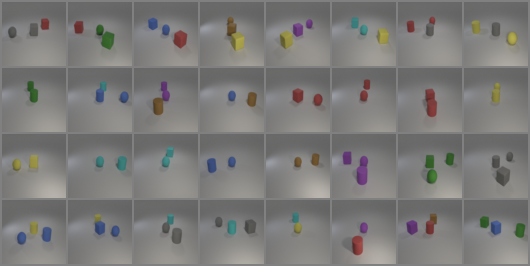
\includegraphics[width=\textwidth]{figures/new_test_result.png}
        \caption{new\_test.json 的生成結果}
        \label{fig:new_test_result}
    \end{subfigure}
    \vspace{1em} % 此指令用於在兩個子圖之間產生垂直間隔
    \begin{subfigure}[b]{0.8\textwidth}
        \centering
        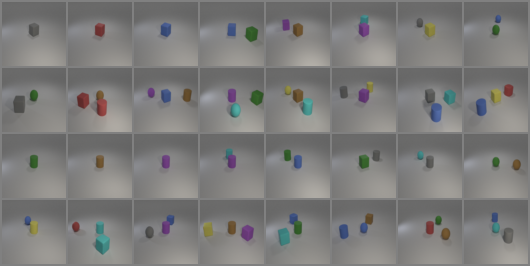
\includegraphics[width=\textwidth]{figures/test_result.png}
        \caption{test.json 的生成結果}
        \label{fig:test_result}
    \end{subfigure}
    \caption{模型為 test.json 與 new\_test.json 生成的合成圖像。}
    \label{fig:synthetic_images_grids}
\end{figure}

為了更深入地理解模型的學習過程,我進一步展示了在不同訓練階段(epochs)下,模型對於特定標籤組合 ``red sphere'', ``cyan cylinder'', ``cyan cube'' 的去噪過程。圖 \ref{fig:denoising_process} 由上至下依序呈現了模型在訓練了 100、500、2500 及 2700 個 epoch 後的去噪結果。從這些圖像中,我可以觀察到隨著訓練的進行,模型一開始是什麼都沒有學會,然後先生成了與方塊還有圓柱相似的物體,而且擺在圖片的後面,然後才學會放到圖片前,強調出稜角與圓角。

\begin{figure}[H]
    \centering
    \begin{subfigure}[b]{0.8\textwidth}
        \centering
        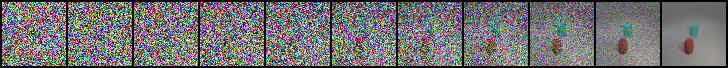
\includegraphics[width=\textwidth]{figures/ep100_25.png}
        \label{fig:ep100_25}
    \end{subfigure}
    \vspace{1em}
    \begin{subfigure}[b]{0.8\textwidth}
        \centering
        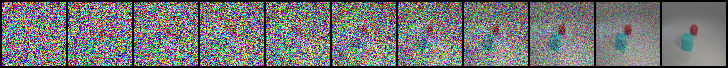
\includegraphics[width=\textwidth]{figures/ep500_25.png}
        \label{fig:ep500_25}
    \end{subfigure}
    \vspace{1em}
    \begin{subfigure}[b]{0.8\textwidth}
        \centering
        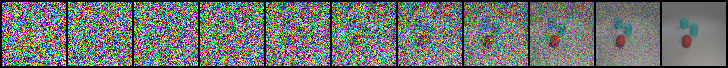
\includegraphics[width=\textwidth]{figures/ep2500_25.png}
        \label{fig:ep2500_25}
    \end{subfigure}
    \vspace{1em}
    \begin{subfigure}[b]{0.8\textwidth}
        \centering
        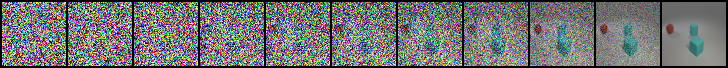
\includegraphics[width=\textwidth]{figures/ep2700_25.png}
        \label{fig:ep2700_25}
    \end{subfigure}
    \caption{不同訓練階段的去噪過程比較,標籤為 ["red sphere", "cyan cylinder", "cyan cube"]。從上到下分別為 epoch 100、500、2500 和 2700 的去噪過程。}
    \label{fig:denoising_process}
\end{figure}

\subsection{Evaluate your model with the classification accuracies}

除了視覺上的評估,我也使用了分類準確率來量化模型的性能。圖 \ref{fig:accuracy_plot} 展示了模型在測試集上的分類準確率隨訓練過程的變化,在接近 30 小時的訓練之後,我在 epoch 2700 時,得到了 98 \% 的準確率。

\begin{figure}[H]
    \centering
    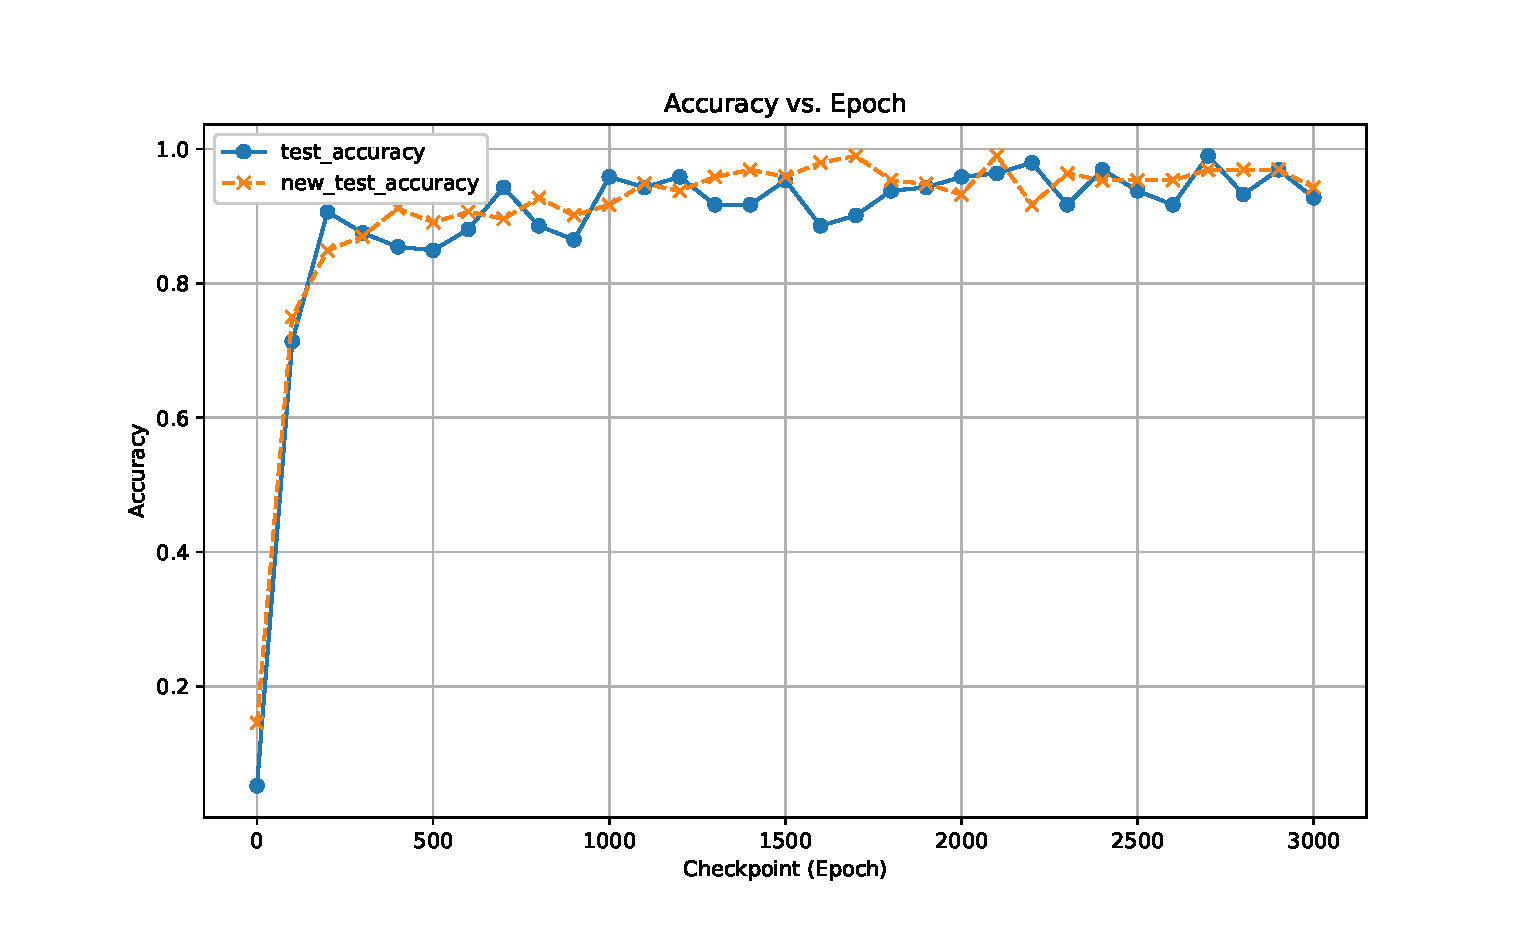
\includegraphics[width=0.8\textwidth]{figures/accuracy_plot.eps}
    \caption{模型在測試集上的分類準確率}
    \label{fig:accuracy_plot}
\end{figure}

\begin{figure}[H]
    \centering
    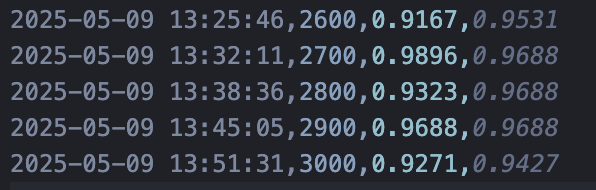
\includegraphics[width=0.8\textwidth]{figures/accuracy.png}
    \caption{模型在測試集上的分類準確率}
    \label{fig:accuracy}
\end{figure}


\subsection{Extra implementations and experiments: Training Details}

在一開始訓練的時候,當固定 epoch 的時候,會發現 batch size 越小的訓練 loss 越低,這讓我非常的困惑,那為什麼所有的論文都說 batch size 越大越好呢? 所以我猜測雖然 batch 小的收斂快,但是可能很容易卡在比較高的 local minimum,沒辦法更進一步,又或是因為 batch 比較小,所以會有很多次 update model 的機會,導致模型在訓練過程中,會有比較多的機會,可以更新模型,這樣可以讓模型學習到更多的資訊?

所以我固定了更新模型的次數,想要比較 batch\ size 16 vs 160 的差異,但是我發現我的電腦沒辦法訓練 batch 160,所以這裡我實作了 amp。圖~\ref{fig:different_bz} 初步展示了在不同 batch\ size 設定下訓練過程的比較,這有助於我理解 batch\ size 對模型學習效率和最終性能的潛在影響。

\begin{figure}[H]
    \centering
    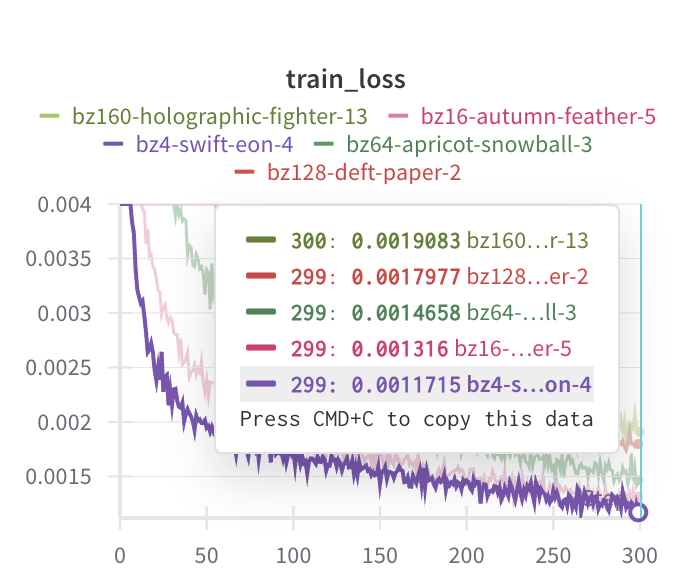
\includegraphics[width=0.8\textwidth]{figures/different_bz.png}
    \caption{不同 batch size 的訓練過程比較}
    \label{fig:different_bz}
\end{figure}

讓模型可以在 4090 的 24 G 記憶體上,訓練到 160 個 batch\_size,最終的結果也沒有辜負我的期望,可以在 41 秒跑完一個 epoch,這裡我訓練了 3000 個 epoch,可以達到 0.98 的準確率,會設計 3000 個 epoch 的原因是,batch 16 的 會比 batch 160 多更新模型 10倍的次數,這很明顯會對於 big batch 不利,所以我選擇讓更新的數量一樣,可以比較公平的比較。圖 \ref{fig:bz16vs160} 更細緻地比較了 batch size 為 16(子圖 \ref{fig:bz16_1})與 batch size 為 160(子圖 \ref{fig:bz16_2})時的訓練過程。透過這組比較,我可以更清晰地觀察在固定模型更新次數的前提下,不同 batch size 對訓練動態(如損失函數的下降速度、穩定性等)以及最終模型性能的具體差異。

\begin{figure}[H]
    \centering
    \begin{subfigure}[b]{0.48\textwidth}
        \centering
        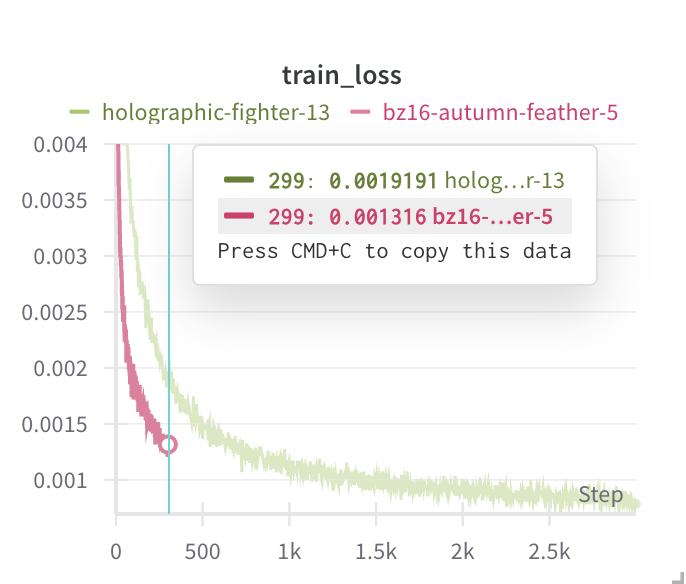
\includegraphics[width=\textwidth]{figures/bz16vs160_1.png}
        \caption{batch size 16 的訓練過程}
        \label{fig:bz16_1}
    \end{subfigure}
    \vspace{1em}
    \begin{subfigure}[b]{0.48\textwidth}
        \centering
        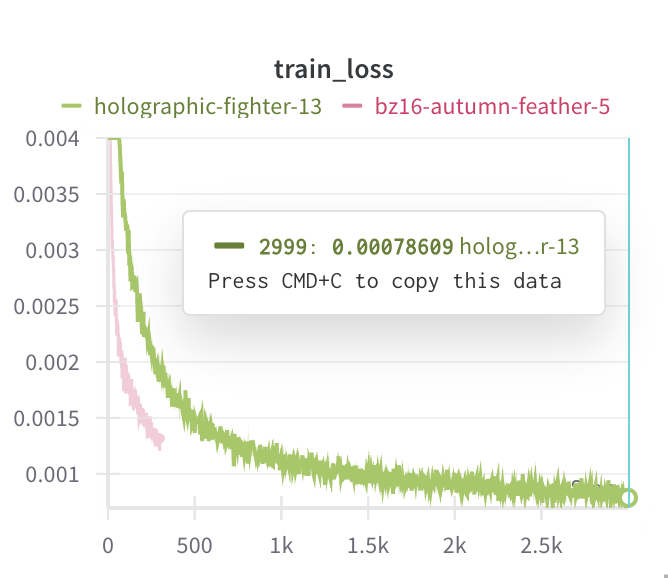
\includegraphics[width=\textwidth]{figures/bz16vs160_2.png}
        \caption{batch size 160 的訓練過程}
        \label{fig:bz16_2}
    \end{subfigure}
    \caption{不同 batch size 的訓練過程比較}
    \label{fig:bz16vs160}
\end{figure}






% 添加參考文獻
\clearpage
\printbibliography

\end{document} 